\documentclass[11pt]{article}
\usepackage[a4paper,margin=2.8cm]{geometry}
\usepackage{amsfonts}
\usepackage{mathtools}
\usepackage{cancel}
\usepackage{amsthm}
\usepackage{amsmath}
\usepackage{amssymb}
\usepackage{dsfont}
\usepackage[dvipsnames,usenames]{color}
\usepackage[colorlinks=true,linkcolor=NavyBlue,citecolor=NavyBlue,urlcolor=NavyBlue]{hyperref} % for hyperlinks 
\usepackage{floatpag} % remove page number for figure that covers entire page

% macros 
%%%%%%%%%%%%%%%%%%%%%%%%%%%%%%%%%%%%%%%%%%%%%%%%%%%%%%%%%%%%%%%%%%%%%%%%%%%%
\newcommand{\R}{\mathds {R}}
\newcommand{\red}[1]{\textcolor{WildStrawberry}{#1}} % for color for remarks
\newcommand{\green}[1]{\textcolor{Green}{#1}} % for color for remarks


\title{Fair, Stable Exchange Networks through Quenched Merchant Location and Idiosyncratic Trading Costs}

\author{Nate Dwyer, Sandro Lera, and Alex `Sandy' Pentland}

\begin{document}

\maketitle
\setcounter{section}{0}

\section*{Extended Abstract}

Until not too long ago, people used to live in more self-contained villages,
with local markets where people buy different products.  Take clothing as an
example. Most villages had one or several clothing merchants competing for
customers.  There is some healthy competition among merchants within a village,
as people can flexibly switch according to prices and preferences. But
customers would rarely buy clothing from a faraway village, as the transaction
cost associated with visiting that village would be high,  and could not offset
a marginally better price or quality.  On the other hand, people living far
away from any village are disadvantaged as they always incur such high costs.
Similarly, if there is a specialized product that can only be produced in some
villages, it was harder to find customers across village borders,  making it
more difficult for new products and technologies to succeed. 

From the industrial to the technological revolution, more efficient
distribution channels have emerged, enabling people to buy almost any product
in online stores.  Independent of a customer's physical location, orders can be
delivered to their door within a day.  More specialized products are now sold
globally, and people living far away from hubs benefit from the availability of
a wide range of products.  While such efficiency is beneficial for the economy
as a whole, it comes at the cost of potential monopolies.  Consider a merchant
that manages to sell a product for a few cents cheaper than its competitors. 
Given modern distribution channels, and ignoring potential differences in
quality, every buyer is now incentivized to buy from that one firm at the
cheaper price. One potential outcome is that the competitors follow along,
increase their efficiency, and a new equilibrium is reached.  However, in a
suboptimal scenario, that one firm leverages the temporarily increased revenue
to further outpace and potentially undercut its competitors.  In the short
term, feedback mechanisms kick in, and an initially minor gap in competitive
advantage, mixed with efficient distribution channels, manifests itself in a
monopoly situation. 

We conclude that geographical constraints can lead to unfair and inefficient
conditions for the customers, whereas removal of those constraints can lead to
exploitative monopolies.

In this work, we introduce an individualized tax between buyers and firms based
on distance. Through tuning of this tax and targeted redistribution of tax
money to regions of low economic activity, we show that this model is able to
[put conclusions here, everything else right now is speculation.]

\section{Introduction}
Consider competing firms in a number of small towns. Each town wants to
encourage their local firm to succeed, but at the same time does not want for
its citizens to face monopoly prices. Hence, the towns all levy small,
percentage sales taxes on out of town goods. These taxes increase as the origin
of the good gets more distant.

In addition, the firms that initially do well tend to get better and better
over time and build up an advantage over other firms. This is especially true
with network based firms, where quality of the product is dwarfed by quantity
of the network. 

With enough market power, a profit seeking firm will try to raise barriers to
entry to prevent competition. This stops firms that have new innovations from
surviving long enough to succeed in a market. The distance based tax introduced
in this paper allows start ups to overcome entrenched monopolies' unfair
advantages.

In this paper, we propose a new distance based tax, which we call an
idiosyncratic tax, in order to solve these
problems, then show that it works by modelling an economy that implements the
tax. In section 2 we give an overview of this economy. In section 3 we
formalize the model, and discuss how the firms compete on capacity and price.
In section 4 we expand the model by allowing for multiple timesteps, and having
firms decrease their costs based on previous profits as a form of investment.

\section{Economy}
We simulate an economy of buyers and firms in some environment with a distance
(e.g. a country, a network economy). Then we apply the idiosyncratic tax that
increases with distance of purchase and see how firms respond. 

\subsection{Geography}
The geography of our model is one-dimensional with periodic boundaries, i.e.
a topological circle, of length $L$. Due to the periodic boundary conditions,
we measure physical distances with the metric $\min(|x-y|, L-|x-y|)$ for any
two points (`agents') $x$,$y$ on the circle. Without loss of generality, we set
$L=1$. Our model does not rely on the implemented geography, and any other,
potentially more realistic topology could be considered.

The left insets (subgraphs (a), (c), (e), (g), and (i)) of Figure
\pageref{fig:fig3x2SingleTimestep} are examples of such a geography.

\subsection{Buyers}
We randomly place buyers on the circle. Each buyer tries to buy as much product
as possible, while constrained by a demand curve that limits how much they can
buy at given prices. 

\subsection{Firms}
The firms, like the buyers, are also randomly placed on the circle, and compete
non-cooperatively to maximize their profit. Each firm makes two choices, first
capacity (i.e. how much they produce), then price, in order to earn the most
profit. A firm chooses capacity before price because it is difficult to quickly
change capacity due to supply chain restraints, while it is easier to change a
price tag.

\subsection{Idiosyncratic Tax}
[talk about new product means d=1 for everyone]
The idiosyncratic tax that is introduced by this paper is dependent on 
discrete distance metric [need another term] $D$ between a buyer and a firm,
where the closest firm to a buyer is at distance $D=1$, the next closest at
$D=2$, and the $n$th closest at $D=n$. Consider a firm and two buyers, one
buyer near the firm, the other distant. The idiosyncratic tax means that the
nearer buyer can buy more cheaply from that firm than can the more distant one.
This incentivizes buyers to purchase from more local firms.

Crucially, this discrete distance metric is calculated for every type of
product individually. This means that a dentist and a bakery do not increase
each other's distance from their buyers. In addition, this means that if a firm
produces a new product, such as a new drug, it is considered at distance 1 from
all buyers, until a competitor emerges.

\section{Model Definition}
When firms choose capacity and price, they make their choices in order to
maximize profit. First, the firms compete on a capacity, by simultaneously
declaring how much of the product they plan to produce; next, they compete on
price to determine the firms' non-tax prices. This process, consisting of these
two subgames is called a Kreps-Scheinkman game. The major difference we
introduce to the classical Kreps-Scheinkman game is the idiosyncratic tax,
which significantly alters the pricing subgame.

\subsection{Capacity Game}
The first choice is how much capacity $\hat q_i$ each firm $i$ wishes to
install. The firm's desire to increase capacity is limited by two factors.
First, firm $i$ incurs a unit price of $c_i$ for every unit of product they
install, regardless of whether or not the product is sold. Second, because the
buyers have a limited demand, eventually the buyers will stop buying.

The capacity subgame acts much like a Cournot game.\footnote{A Cournot game is
where firms compete only on quantity, and sell all of the quantity at the
market clearing price.} The difference, in our case, is that instead of being
assigned a market clearing price and selling everything they produce, in our
model the firms compete on price in a second subgame where they choose a price.
Only after that do the buyers determine how much of each firms capacity is
sold.

\subsection{Pricing Game}
Each firm $i$, having chosen a capacity $\hat q_i$, now choose a price, $p_i$.
Consider two vending machines selling the same soda right beside one another,
with one machine selling soda at a cheaper price than the other. In this
subgame, buyers will use the cheaper machine first, but if the buyers demand
more soda than the machine's capacity, buyers switch to the more expensive
machine when the cheaper one runs out of soda. Competition on price in such a
manner is called an Edgeworth game. Edgeworth games are very difficult to find
an equilibrium in, as depending on demand and capacity, a variety of optimal
strategies can be employed.

By choosing a lower price, a firm can undercut competitors, ensuring that
buyers choose to buy from them instead of other firms. In addition, because
of the negatively sloped demand curves of buyers, a lower price increases the
amount of product purchased in total. But the capacity limitation on total
quantity sold by a firm means that a single firm usually can't sell to the
entire market, and it could be more profitable to just sell a few at a much
higher price.

\subsection{Idiosyncratic Tax}
An additional complication to the pricing game is the idiosyncratic tax, as it
causes buyers to have preferences for certain firms. The tax is designed to
promote buyers purchasing locally, by having no tax if a buyer purchases from
the nearest firm, and then increasing the tax in discrete steps as firms get
more and more distant. Since each buyer-seller pair has a different tax, the
tax can cause two buyers to perceive separate prices at the same firm.

For any buyer $b$ and firm $i$, we define a product-distance $D = D(b,i)$ such
that the firm $i$ that is physically closest to $b$ has distance $D(b,i)=1$,
the next closest has distance $D=2$, and the $n$th closest has distance $D=n$. 
Thus, if buyer $b$ buys from firm $i$, the total price, including transaction
cost (tax), is given by $p(b,i) = p_i \cdot (e(D(b,i)^\gamma -1) + 1)$ where
$\gamma$ is the scaling coefficient of the tax.

Implementing the distance based tax gives the buyers individualized preferences
over the firms. For example, imagine two firms $i$ and $j$, and let $p_i <
p_j$. Without any tax, every buyer prefers buying from $i$ versus buying from
$j$. But with the tax, this could change. Say that buyer $b$ is very close to
firm $j$, and very far from firm $i$, so that $D(b,i)^\gamma \gg
D(b,j)^\gamma$. Then buyer $b$ would prefer to buy from $j$ despite $j$'s price
being higher because $p_i\cdot D(b,i)^\gamma > p_j\cdot D(b,j)^\gamma$.

This gives rise to two interesting limit cases, one where $\gamma = 0$, and the
other where $\gamma = \infty$.  When $\gamma = 0$, no firms are taxed anywhere,
so the game simplifies into a pure Kreps-Scheinkman game. In contrast, when
$\gamma = \infty$, it becomes impossible for buyers to purchase from non local
firms, and so the firms all impose monopolistic prices.

\subsection{Buyer Behavior and Rationing}
After the firms have finished determining capacity and price, and the distance
based tax has been incorporated into the prices, the buyers conduct purchases
as follows.

Let the set of buyers be called $B$. Each buyer $b\in B$ buys a quantity $q_b =
\sum_{i\in S} q_{b,i}$, where $q_{b,i}$ is the amount buyer $b$ buys from the
firm $i$. The buyer's all have identical demand curves $p_\text{max} + q_b =
a$, where $a$ is the endowment they are given exogenously, and $p_\text{max}$
is the maximum price they pay (including tax). Each buyer tries to maximize
$q_b$ while keeping $P + Q \le a$. In other words, they buy from the cheapest
available firm until they hit the demand curve.

If a buyer perceives multiple firms as offering identical prices, they buy from
all such firms in identical amounts until either the buyer hits their demand
curve, or a seller runs out of capacity. 

\subsection{Profit Function}
Finally, firm $i$, having chosen quantity $\hat q_i$ and price $p_i$, and
having sold the product to buyers, will earn a profit:

\begin{equation}
    \Pi_i = p_i\sum_{b\in B} q_{b,i} - c_i\hat q_i.
\end{equation}

Note that while the firm can choose both their capacity $\hat q_i$ and their
price $p_i$, their cost per unit $c_i$ is set exogenously. Also, each $q_{b,i}$
is chosen by the buyer $b$ so that they buy as much as possible while staying
under their demand curve $P+Q\leq a$; this is where taxes affect the firm's
profit.

If the firm sells all of their capacity, the equation simplifies to:
\begin{equation}
    \Pi_i = (p_i- c_i)\hat q_i,
\end{equation}
which is the profit per unit multiplied by quantity sold, which is the same as
capacity.

\section{Model Solution and Examples}

\subsection{Numeric Solution}
Because the buyers have individualized preferences and the pricing game does
not necessarily have a pure Nash equilibrium, it is difficult to determine a
generalized, theoretical Nash equilibrium to the model laid out is section 3.
Instead, we determine the Nash equilibrium numerically.

First we discretize the possible strategies the firms can take, so we only have
to consider a finite number of strategies.

We would like to determine what the Nash quantity is, but we do not currently
know what the payoff for particular combinations of strategies until we
determine price. So we need to start by determining the Nash prices for every
combination of quantities, which we do by using the Python library Gambit,
which can solve game theoretic questions. We use the price choices to determine
the payoffs of capacity choices. Finally, we use Gambit again to determine what
the Nash capacity is.

We work backwards. First we find the payoffs for all of the possible prices
given capacity. Then we use the Python library Gambit to determine the Nash
equilibrium price. Now if the firms make the same capacity choices, then they
will make

Besides the basic geometry of the model, in order to determine how much profit
a firm makes we need to know how much capacity every firm produces and what
prices they sell at. But this presents a problem, as firms must pick capacity
before choosing price, yet they need to know the price to calculate the profit.

, so we have to first determine the equilibrium price for
each outcome of the 

So we need to determine the prices firms will choose for
every contingency of the capacity game.
prices will be chosen when they choose capacity. This makes it difficult for
them to optimize which capacity to choose. The solution to this is to work
backwards. The firms first find the equilibrium price choice for every
combination of capacity choices that might occur. Then they calculate the
payoffs for every outcome of the capacity game. Finally, we determine the Nash 

Figure \pageref{fig:fig3x2SingleTimestep}, Row 1, has two firms with the same
cost per unit, and $\gamma=0$. To solve this, we first discretized the
capacities and prices firms could choose. Then for each combination of
capacities chosen by Firms 1 and 2, we found the payoffs for every price they
could choose, creating a payoff matrix. Specifically, given that Firm 1 chose
capacity $\hat q_1$ and Firm 2 chose $\hat q_2$, if the firms choose prices
$p_1$ and $p_2$, they will earn profits $\Pi_1$ and $\Pi_2$. After calculating
this for every combination of prices, we then find the Nash equilibrium of the
pricing game. 

we found both firms Nash prices. We then used the knowledge of what the optimal
price was to calculate the 

To do this, 
Next, we need to simulate buyers that try to
purchase goods on the 

Next, since there are two choices, we work backwards to determine the Nash
equilibrium of the game. 

set of capacity strategies $\{\hat q_1, \hat q_2, \cdots, \hat q_{|S|}\}$, we
determine the nash prices $\{p_1, p_2, \cdots, p_{|S|}\}$.  Thus we assemble
the game of 

The firm makes two choices, first capacity, then price. To solve, we first
figure out the nash pricing strategy given 

because it is equivalent
to an Edgeworth game
[elaborate more on edgeworth game in section above, say that this makes it a
mixed nash equilibria] game

\begin{figure}[[p!htb] % p stands for 'entire page', '!htb' is to insert as close to code as possible
	\floatpagestyle{empty} % remove page number
	\centering
	\vspace{-2cm} % shift upwards to get more space for caption
  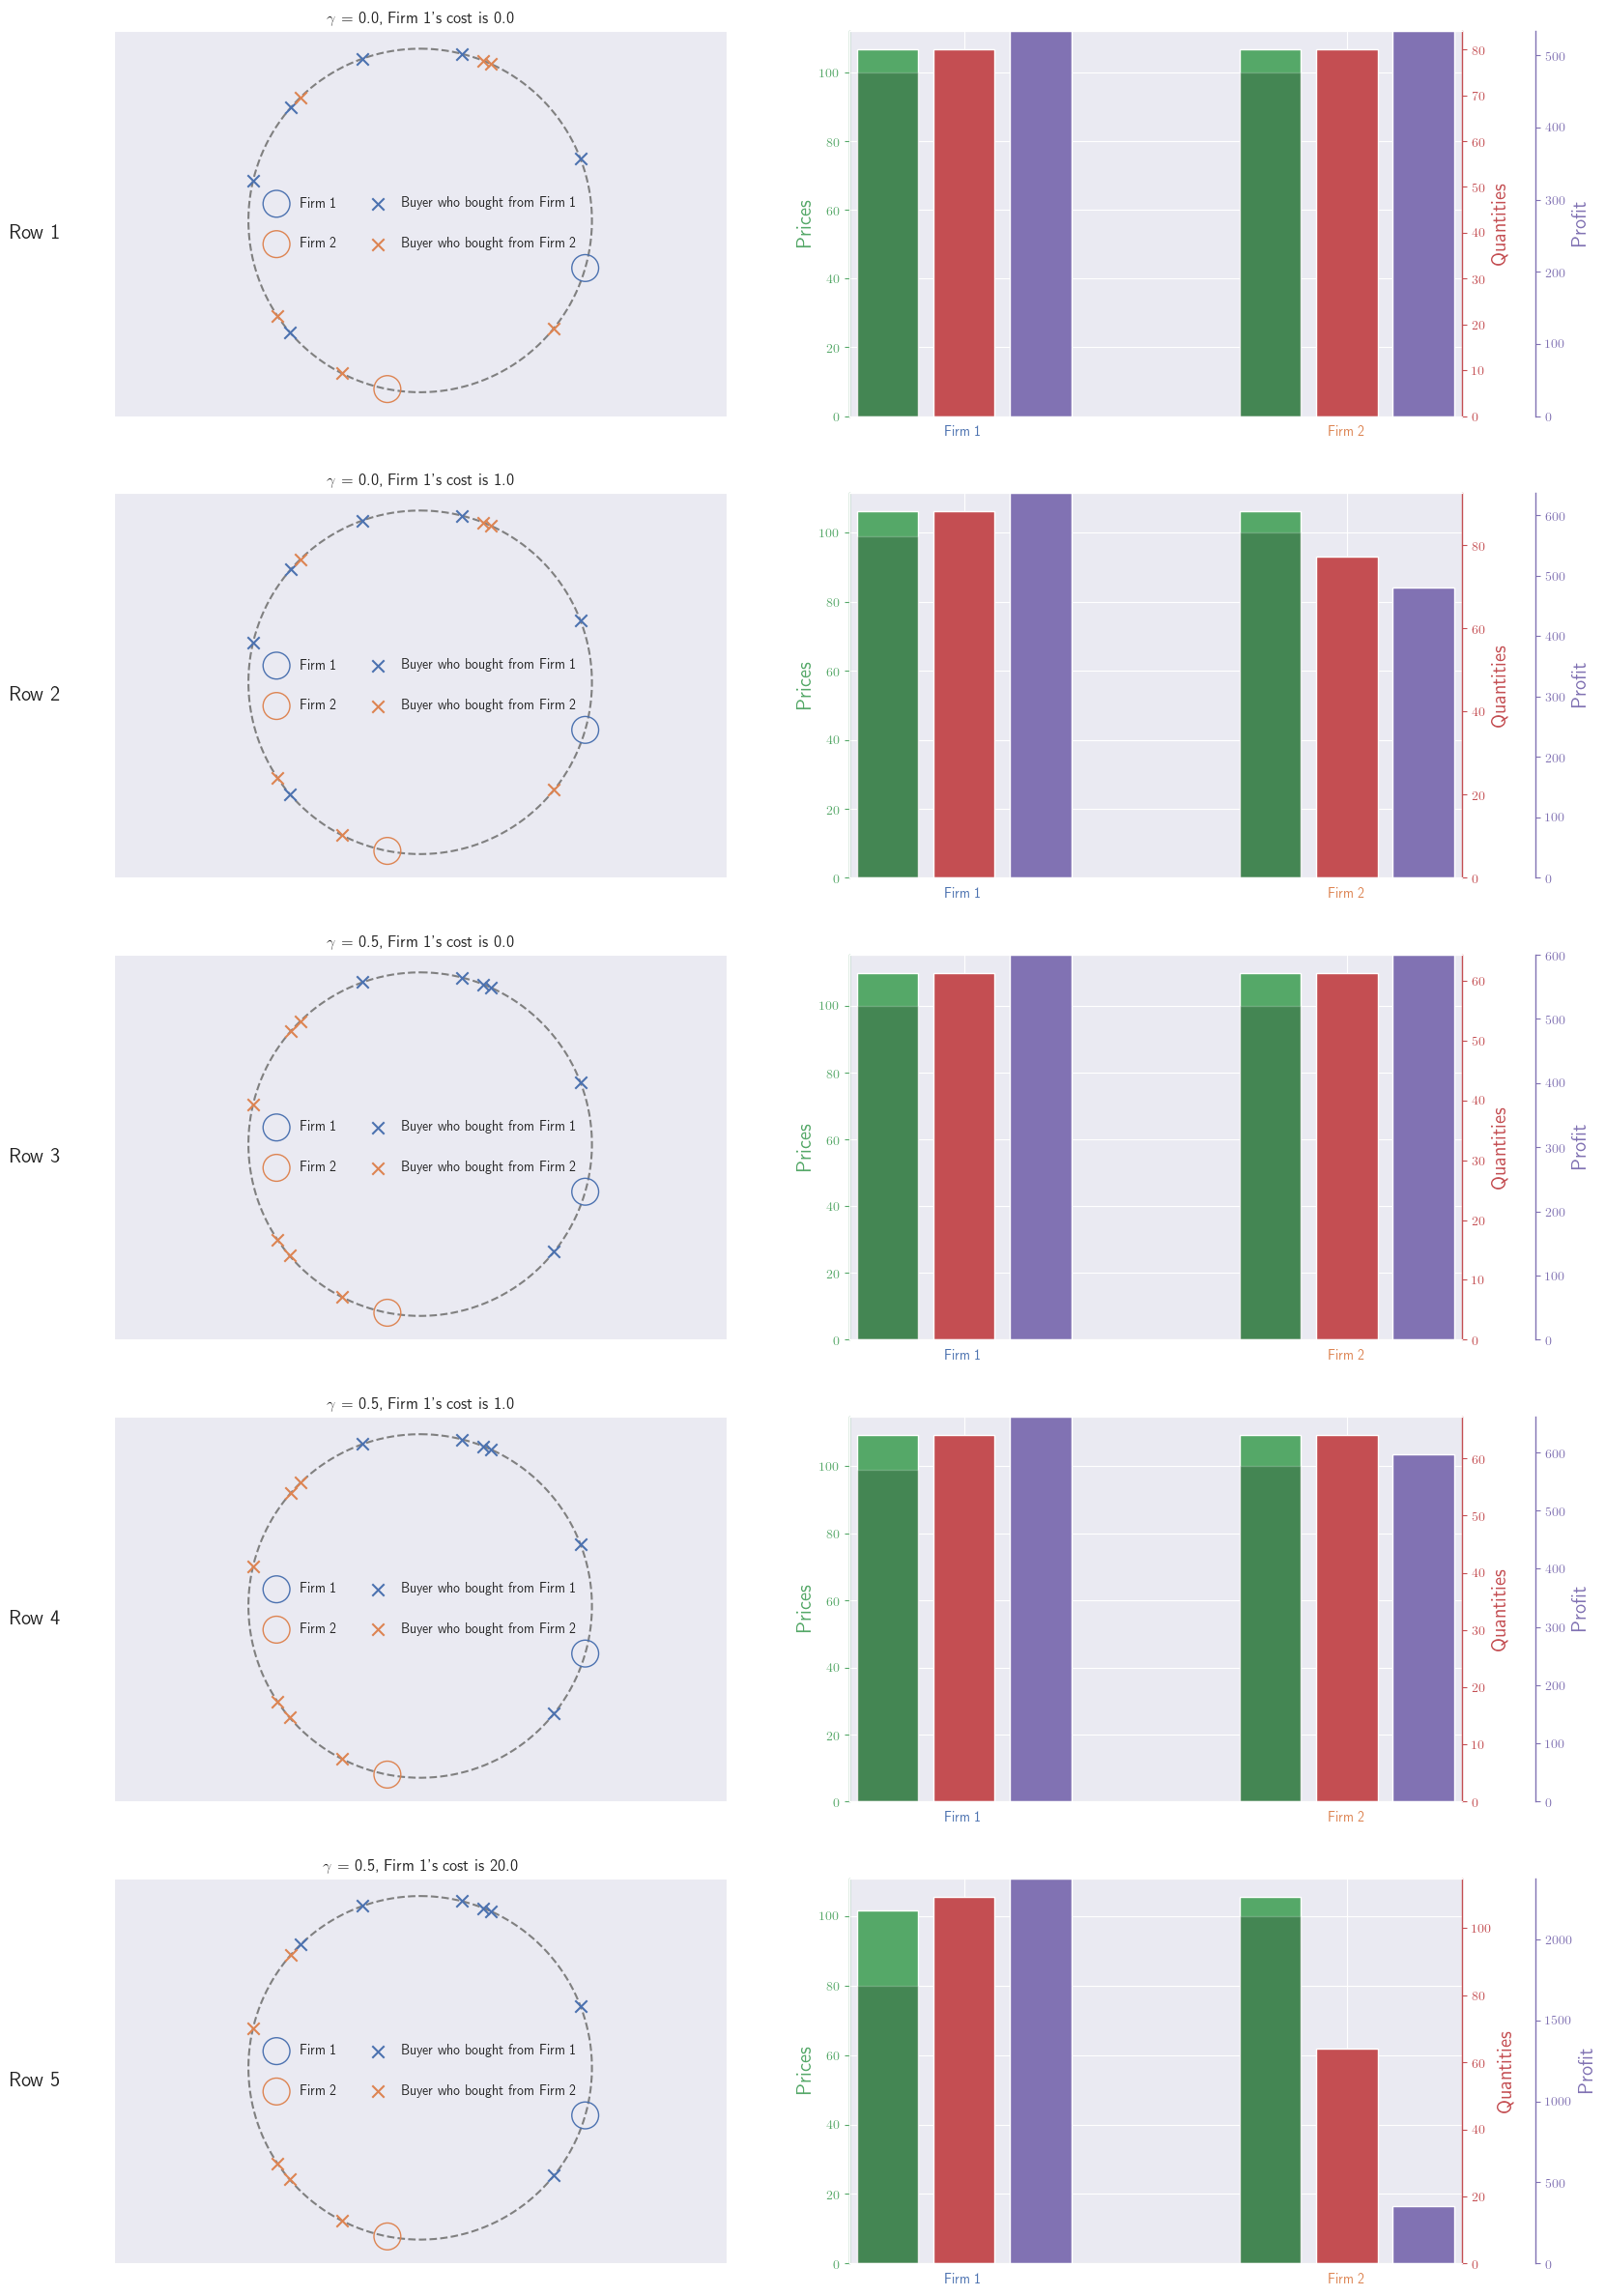
\includegraphics[width=\linewidth]{5x2plot.png}
  \caption{\small{Shown above are five instances of the model running for different
  $\gamma$ and costs. In the first two rows, $\gamma=0$, with the one
  difference being that in Row 1, both Firm 1 and Firm 2 have the same cost,
  and in Row 2, Firm 1 has a 1\% lower cost than Firm 2. In Row 1, the firms
  sell the same amount of product and make the same amount of profit. But in
  Row 2, Firm 1 sells 33\% more quantity and makes 53\% more profit.
  In the rest of the plots, $\gamma = .6$. In Row 3 we can see a mirror of Row
  1, where both firms, faced with the same costs, produce the same quantity,
  and make the same profit. But in row 4, where we give Firm 1
  the same advantage we game them in the row 2, they sell the same amount, and
  only make 12\% more profit than Firm 2. To increase their market share,
  Firm 1 needs to reduce their costs to 80\% of Firm 2, as shown in row 5.
  Our idiosyncratic tax thus acts as a speed bump, preventing companies with
  slight advantages from acquiring overwhelming market dominance, while still
  ensuring that minor innovations are profitable, and that large innovations do
  cause market dominance.}}
  \label{fig:fig3x2SingleTimestep}
\end{figure}




\section{Dynamics}
We run this model once for every timestep, then update the costs for the firms
between the timesteps. Every timestep we determine which firm has made the most
profit. For that firm, we reduce its cost per unit by 5\% in order to simulate
the company investing its excess profits in itself to become more profitable in
the long term. 

[put picture here when done running].

\section{Special Case when $\gamma = 0$}
If $\gamma = 0$, then the tax rate $(D^\gamma - 1) = 0$, which turns the game
into a Kreps-Scheinkman game with firms experiencing different cost functions. 
Theoretically, when per-unit costs are sufficiently close [define sufficiently
close, need to examine judo economics thing for this], the theoretical
Nash ends up being the same as a Cournot game with the same demand curve
and costs [citation].

In our model, we can see that the price predicted by the Cournot model and our
model coincide for most costs. But once the cost get too disparate, the Cournot
model splits from our model. [need explanation for this, possible judo econ
related.] In addition the most

\begin{figure}
  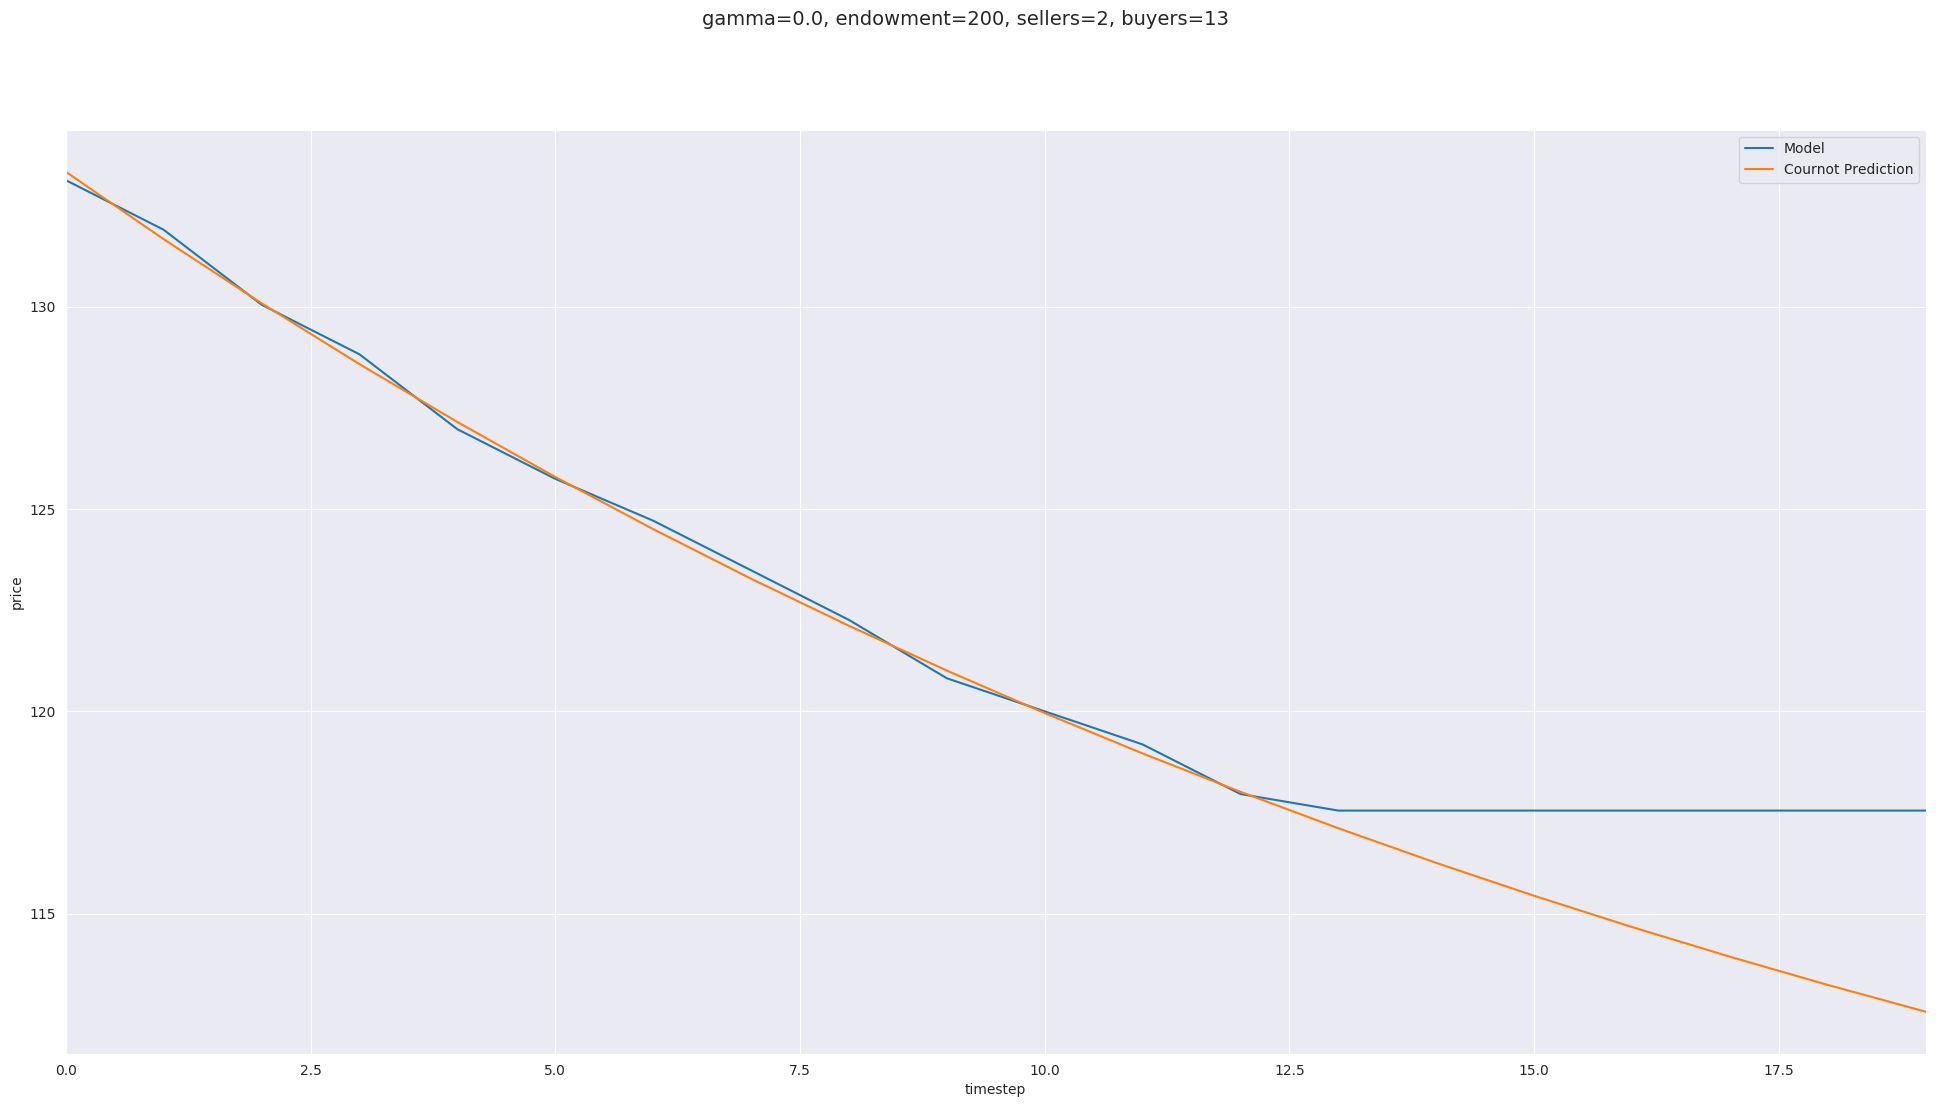
\includegraphics[width=\linewidth]{CournotVsModel.png}
  \caption{A comparison between prices predicted by two models. In blue is the
  one predicted by this paper's numeric approximation of the Kreps-Scheinkman
  model and in orange is the one predicted by the Cournot model.}
  \label{fig:figCournotVsModel}
\end{figure}

\section{Special Case when $\gamma = \infty$}
When $\gamma = \infty$, no buyer can afford any positive price from a non local
firm. Because of this, all firms will charge monopoly prices.

\subsection{What $\gamma$ will cause monopolistic behavior?}
A firm will price at monopoly prices if it knows that it cannot be profitably
undercut, and, conversely, cannot profitably undercut its opponent. So the
question then becomes, at what $\gamma$ do we know that this will hold for all
firms?

We start by finding the maximum price that cannot be profitably undercut.
Consider a firm $i$ trying to determine if it can undercut a competitor. The
firm $i$ will want to make a profit, and thus must sell at a price $p_i > c_i$.
In addition, the least tax a non local buyer would incur purchasing from them
is $2^\gamma$. Thus firm $i$ cannot make a profit if it offers a price $p_i
\leq c_i 2^\gamma$, and if firm $j$ offers a price of $p_j=c_i2^\gamma$, firm
$i$ cannot undercut firm $j$. To a price that no firm can undercut, we find the
minimum value of $c_i$, which we call $c_\text{min}$, for all firms $i\in S$,
leaving us with the conclusion that the maximum price that cannot be profitably
undercut is:

\begin{equation}
  p_\text{max} = c_\text{min}2^\gamma.
\end{equation}

Now we just need to substitute $p_\text{max}$ for the largest monopolistic
price to ensure no firm can be undercut. In general, the monopolistic price for
a firm $i$ with a demand curve of $p_i = a-bq_i$ is $\frac{a+c_i}{2}$ [ref].
Thus the highest monopoly price is $\frac{a+c_\text{max}}{2}$, and we get the
following:
\begin{align}
  c_\text{min}2^\gamma &= p_\text{max}\\
  c_\text{min}2^\gamma &= \frac{a+c_\text{max}}{2}\\
  2^\gamma &= \frac{a+c_\text{max}}{2c_\text{min}}\\
  \gamma &= \frac{\ln(\frac{a+c_\text{max}}{2c_\text{min}})}{\ln(2)}\\
  \gamma &= \frac{\ln(a+c_\text{max}) - \ln(2) -\ln(c_\text{min})}{\ln(2)}
\end{align}

Thus when $\gamma$ satisfies (8), the firms all charge monopoly prices, and act
in the same way as they do when $gamma = \infty$.

\section{Nash Equilibrium of the game}
The analytic solution is unfortunately very difficult to compute for a number
of reasons. First, we must determine the prices firms will choose given their
choice of capacity. This is difficult to do as Edgeworth game does not
necessarily have a pure Nash solution, and it is beyond my abilities to
calculate what the mixed Nash is on a continuous game.  

Fortunately, what our program does is calculate a numeric approximation of what
the Nash equilibrium is for our model. It does this by implementing our model
on a discrete set of strategies for both a firm's capacity and price, and then
solving these games using the program Gambit.

Interestingly, most of the time, the approximate Nash as calculated by the
program usually predicts that [blank here].


\section{Unequal tax model}
Consider a Cournot economy of $n$ firms where the $i$th firm is uniquely
subject to an ad valorem, or percentage, tax at rate $t$, with all other firms
assigned no tax. If there was no tax for firm $i$,  we could describe its
profit function using the equation $\Pi_i(q_i) = q_i(p-c_i)$, where $q_i$ is
the firm's quantity, $p$ the market clearing price, and $c_i$ the product's
unit cost.  The market clearing price is $p = a - bQ$, where $a$ is the
endowment, $b$ the slope of the demand curve, and $Q$ is the total quantity
produced by all firms. By $Q_{-i} = Q - q_i$ we denote the sum of all sold
quantities except $q$. 

Since the firm is subject to a tax, it will have to offer a lower pre-tax
price to match the market clearing price; hence the pre-tax price is
$p_\text{pre-tax} = p/(1+t)$. Factoring this into the profit function gives:

\begin{subequations}
\begin{align}
    \Pi_i &= q_i \left(p_\text{pre-tax} - c\right)\\
          &= q_i \left(\frac{p}{1+t} - c\right)\\
          &= q_i \left(\frac{a - bQ}{1+t} - c\right)\\
          &= q_i \left(\frac{a - b(q_i + Q_{-i})}{1+t} - c\right).
\end{align}
\end{subequations}

Now, to find the best response function (BRF), we take the derivative and
set it to 0:
\begin{subequations}
\begin{align}
    \Pi_i &= q_i \left(\frac{a - b(q_i + Q_{-i})}{1+t} - c\right)\\
    \frac{\mathrm{d}\Pi_i}{\mathrm{d}q_i} &= \frac{a - b(2q_i + Q_{-i})}{1+t} -
    c\\
    0 &= \frac{a - b(2q_i + Q_{-i})}{1+t} - c\\
    0 &= a - b(2q_i + Q_{-i}) - c\left(1+t\right)\\
    2bq_i &= a - bQ_{-i} - c\left(1+t\right)\\
    q_i &= \frac{1}{2b}\left(a-bQ_{-i} - c\left(1+t\right)\right). \label{eq:q_i_unequal_tax_model}
\end{align}
\end{subequations}

We use the BRF's of all the firms to see if they intersect at a common point,
which would be the Nash equilibrium.  In \eqref{eq:q_i_unequal_tax_model},
we can consider the tax as part of the production cost when finding the Nash
quantities, then solve as we normally would a heterogeneous cost Cournot
oligopoly. In other words, taxation is an effective cost.

In a hetereogeneous Cournot economy, the Nash-equilibrium quantity $q_i$
of firm $i$ has cost $c_i$ is given by
\begin{equation}
q_i = \frac{1}{b (n+1)}(a + n(\bar c - c_i) - c_i)\text{,}
\end{equation}
where $n$ is the number of firms, $\bar c$ is the average cost, and $a$ and $b$
come from the demand curve $p = a-bQ$, where $Q$ is total quantity. \red{At
least in a footnote, provide a reference where you got that formula from.}

Interestingly, the BRF we get from a percentage tax is similar to the BRF we
would get if we had a specific tax, also known as a per unit tax.  A specific
or per unit tax is one that adds a flat extra cost per unit created,
effectively increasing the cost by a fixed amount. Say the specific tax was
$t_\text{specific}$. Then the profit function would look like:
\begin{equation}
\Pi = q (p-c-t_\text{specific})
\end{equation}
and the BRF would be:
\begin{equation}
q = \frac{1}{2}(a-q_\text{other} - c - t_\text{specific})
\end{equation}
which means that we could again just consider $c - t_\text{specific}$ as the
cost that the firm faces, and also solve as normal.  


\section{Open Questions}

\begin{itemize}

    \item With this model, we want to demonstrate that initially small
        differences in quality do not lead to proportional feedback mechanisms
        that lead to an unequal output distribution So it might be questionable
        if the current Cournot model is the model of our interests, because it
        assumes all buyers set the same price. 

\end{itemize}

\subsection{Summary}
The firms play two gamesjcompete first in a Cournot economy where they chose a
capacity, then in a Bertrand-Edgeworth economy where they choose the price.  A
sequential game without the taxes and variable costs is called the
Kreps-Scheinkman model.

\end{document}
